

% Note that the a4paper option is mainly intended so that authors in
% countries using A4 can easily print to A4 and see how their papers will
% look in print - the typesetting of the document will not typically be
% affected with changes in paper size (but the bottom and side margins will).
% Use the testflow package mentioned above to verify correct handling of
% both paper sizes by the user's LaTeX system.
%
% Also note that the "draftcls" or "draftclsnofoot", not "draft", option
% should be used if it is desired that the figures are to be displayed in
% draft mode.
%
\documentclass[a4paper,conference]{IEEEtran}
% Add the compsoc option for Computer Society conferences.
%
% If IEEEtran.cls has not been installed into the LaTeX system files,
% manually specify the path to it like:
% \documentclass[conference]{../sty/IEEEtran}


% *** MISC UTILITY PACKAGES ***
%
%\usepackage{ifpdf}
% Heiko Oberdiek's ifpdf.sty is very useful if you need conditional
% compilation based on whether the output is pdf or dvi.
% usage:
% \ifpdf
%   % pdf code
% \else
%   % dvi code
% \fi
% The latest version of ifpdf.sty can be obtained from:
% http://www.ctan.org/tex-archive/macros/latex/contrib/oberdiek/
% Also, note that IEEEtran.cls V1.7 and later provides a builtin
% \ifCLASSINFOpdf conditional that works the same way.
% When switching from latex to pdflatex and vice-versa, the compiler may
% have to be run twice to clear warning/error messages.






% *** CITATION PACKAGES ***
%
\usepackage{cite}

% cite.sty was written by Donald Arseneau
% V1.6 and later of IEEEtran pre-defines the format of the cite.sty package
% \cite{} output to follow that of IEEE. Loading the cite package will
% result in citation numbers being automatically sorted and properly
% "compressed/ranged". e.g., [1], [9], [2], [7], [5], [6] without using
% cite.sty will become [1], [2], [5]--[7], [9] using cite.sty. cite.sty's
% \cite will automatically add leading space, if needed. Use cite.sty's
% noadjust option (cite.sty V3.8 and later) if you want to turn this off.
% cite.sty is already installed on most LaTeX systems. Be sure and use
% version 4.0 (2003-05-27) and later if using hyperref.sty. cite.sty does
% not currently provide for hyperlinked citations.
% The latest version can be obtained at:
% http://www.ctan.org/tex-archive/macros/latex/contrib/cite/
% The documentation is contained in the cite.sty file itself.






% *** GRAPHICS RELATED PACKAGES ***
%
\ifCLASSINFOpdf
  % \usepackage[pdftex]{graphicx}
  % declare the path(s) where your graphic files are
  % \graphicspath{{../pdf/}{../jpeg/}}
  % and their extensions so you won't have to specify these with
  % every instance of \includegraphics
  % \DeclareGraphicsExtensions{.pdf,.jpeg,.png}
\else
  % or other class option (dvipsone, dvipdf, if not using dvips). graphicx
  % will default to the driver specified in the system graphics.cfg if no
  % driver is specified.
   \usepackage[dvips]{graphicx}
  % declare the path(s) where your graphic files are
   \graphicspath{{./pics/}}
  % and their extensions so you won't have to specify these with
  % every instance of \includegraphics
   \DeclareGraphicsExtensions{.eps}
\fi


% *** MATH PACKAGES ***
%
%\usepackage[cmex10]{amsmath}
% A popular package from the American Mathematical Society that provides
% many useful and powerful commands for dealing with mathematics. If using
% it, be sure to load this package with the cmex10 option to ensure that
% only type 1 fonts will utilized at all point sizes. Without this option,
% it is possible that some math symbols, particularly those within
% footnotes, will be rendered in bitmap form which will result in a
% document that can not be IEEE Xplore compliant!
%
% Also, note that the amsmath package sets \interdisplaylinepenalty to 10000
% thus preventing page breaks from occurring within multiline equations. Use:
%\interdisplaylinepenalty=2500
% after loading amsmath to restore such page breaks as IEEEtran.cls normally
% does. amsmath.sty is already installed on most LaTeX systems. The latest
% version and documentation can be obtained at:
% http://www.ctan.org/tex-archive/macros/latex/required/amslatex/math/





% *** SPECIALIZED LIST PACKAGES ***
%
%\usepackage{algorithmic}
% algorithmic.sty was written by Peter Williams and Rogerio Brito.
% This package provides an algorithmic environment fo describing algorithms.
% You can use the algorithmic environment in-text or within a figure
% environment to provide for a floating algorithm. Do NOT use the algorithm
% floating environment provided by algorithm.sty (by the same authors) or
% algorithm2e.sty (by Christophe Fiorio) as IEEE does not use dedicated
% algorithm float types and packages that provide these will not provide
% correct IEEE style captions. The latest version and documentation of
% algorithmic.sty can be obtained at:
% http://www.ctan.org/tex-archive/macros/latex/contrib/algorithms/
% There is also a support site at:
% http://algorithms.berlios.de/index.html
% Also of interest may be the (relatively newer and more customizable)
% algorithmicx.sty package by Szasz Janos:
% http://www.ctan.org/tex-archive/macros/latex/contrib/algorithmicx/




% *** ALIGNMENT PACKAGES ***
%
%\usepackage{array}
% Frank Mittelbach's and David Carlisle's array.sty patches and improves
% the standard LaTeX2e array and tabular environments to provide better
% appearance and additional user controls. As the default LaTeX2e table
% generation code is lacking to the point of almost being broken with
% respect to the quality of the end results, all users are strongly
% advised to use an enhanced (at the very least that provided by array.sty)
% set of table tools. array.sty is already installed on most systems. The
% latest version and documentation can be obtained at:
% http://www.ctan.org/tex-archive/macros/latex/required/tools/


%\usepackage{mdwmath}
%\usepackage{mdwtab}
% Also highly recommended is Mark Wooding's extremely powerful MDW tools,
% especially mdwmath.sty and mdwtab.sty which are used to format equations
% and tables, respectively. The MDWtools set is already installed on most
% LaTeX systems. The lastest version and documentation is available at:
% http://www.ctan.org/tex-archive/macros/latex/contrib/mdwtools/


% IEEEtran contains the IEEEeqnarray family of commands that can be used to
% generate multiline equations as well as matrices, tables, etc., of high
% quality.


%\usepackage{eqparbox}
% Also of notable interest is Scott Pakin's eqparbox package for creating
% (automatically sized) equal width boxes - aka "natural width parboxes".
% Available at:
% http://www.ctan.org/tex-archive/macros/latex/contrib/eqparbox/





% *** SUBFIGURE PACKAGES ***
%\usepackage[tight,footnotesize]{subfigure}
% subfigure.sty was written by Steven Douglas Cochran. This package makes it
% easy to put subfigures in your figures. e.g., "Figure 1a and 1b". For IEEE
% work, it is a good idea to load it with the tight package option to reduce
% the amount of white space around the subfigures. subfigure.sty is already
% installed on most LaTeX systems. The latest version and documentation can
% be obtained at:
% http://www.ctan.org/tex-archive/obsolete/macros/latex/contrib/subfigure/
% subfigure.sty has been superceeded by subfig.sty.



%\usepackage[caption=false]{caption}
%\usepackage[font=footnotesize]{subfig}
% subfig.sty, also written by Steven Douglas Cochran, is the modern
% replacement for subfigure.sty. However, subfig.sty requires and
% automatically loads Axel Sommerfeldt's caption.sty which will override
% IEEEtran.cls handling of captions and this will result in nonIEEE style
% figure/table captions. To prevent this problem, be sure and preload
% caption.sty with its "caption=false" package option. This is will preserve
% IEEEtran.cls handing of captions. Version 1.3 (2005/06/28) and later 
% (recommended due to many improvements over 1.2) of subfig.sty supports
% the caption=false option directly:
%\usepackage[caption=false,font=footnotesize]{subfig}
%
% The latest version and documentation can be obtained at:
% http://www.ctan.org/tex-archive/macros/latex/contrib/subfig/
% The latest version and documentation of caption.sty can be obtained at:
% http://www.ctan.org/tex-archive/macros/latex/contrib/caption/




% *** FLOAT PACKAGES ***
%
%\usepackage{fixltx2e}
% fixltx2e, the successor to the earlier fix2col.sty, was written by
% Frank Mittelbach and David Carlisle. This package corrects a few problems
% in the LaTeX2e kernel, the most notable of which is that in current
% LaTeX2e releases, the ordering of single and double column floats is not
% guaranteed to be preserved. Thus, an unpatched LaTeX2e can allow a
% single column figure to be placed prior to an earlier double column
% figure. The latest version and documentation can be found at:
% http://www.ctan.org/tex-archive/macros/latex/base/



%\usepackage{stfloats}
% stfloats.sty was written by Sigitas Tolusis. This package gives LaTeX2e
% the ability to do double column floats at the bottom of the page as well
% as the top. (e.g., "\begin{figure*}[!b]" is not normally possible in
% LaTeX2e). It also provides a command:
%\fnbelowfloat
% to enable the placement of footnotes below bottom floats (the standard
% LaTeX2e kernel puts them above bottom floats). This is an invasive package
% which rewrites many portions of the LaTeX2e float routines. It may not work
% with other packages that modify the LaTeX2e float routines. The latest
% version and documentation can be obtained at:
% http://www.ctan.org/tex-archive/macros/latex/contrib/sttools/
% Documentation is contained in the stfloats.sty comments as well as in the
% presfull.pdf file. Do not use the stfloats baselinefloat ability as IEEE
% does not allow \baselineskip to stretch. Authors submitting work to the
% IEEE should note that IEEE rarely uses double column equations and
% that authors should try to avoid such use. Do not be tempted to use the
% cuted.sty or midfloat.sty packages (also by Sigitas Tolusis) as IEEE does
% not format its papers in such ways.





% *** PDF, URL AND HYPERLINK PACKAGES ***
%
%\usepackage{url}
% url.sty was written by Donald Arseneau. It provides better support for
% handling and breaking URLs. url.sty is already installed on most LaTeX
% systems. The latest version can be obtained at:
% http://www.ctan.org/tex-archive/macros/latex/contrib/misc/
% Read the url.sty source comments for usage information. Basically,
% \url{my_url_here}.





% *** Do not adjust lengths that control margins, column widths, etc. ***
% *** Do not use packages that alter fonts (such as pslatex).         ***
% There should be no need to do such things with IEEEtran.cls V1.6 and later.
% (Unless specifically asked to do so by the journal or conference you plan
% to submit to, of course. )


% correct bad hyphenation here
\hyphenation{op-tical net-works semi-conduc-tor}


\begin{document}
%
% paper title
% can use linebreaks \\ within to get better formatting as desired
\title{Pragmatics Dependent Hardware Design}


% author names and affiliations
% use a multiple column layout for up to three different
% affiliationsy
\author{\IEEEauthorblockN{
Taras Zakharchenko \IEEEmembership{Student Member, IEEE}
}
\IEEEauthorblockA{National technical university of Ukraine\\
``Kyiv polytechnic institute''\\
Ukraine, Kyiv\\
Email: taras@ieee.org}}

% make the title area
\maketitle


\begin{abstract}
%\boldmath
The paper is about hardware design metodology, in which pragmatics of design goal has the most significant influence on design ever. The author describes  basics of pragmatics dependent approach and proposes solution for automated transition from semantic notation of solution of problem given to specific syntaxes, describes its implementation.
\end{abstract}
% no keywords

\IEEEpeerreviewmaketitle

%The Introduction serves to help the reader understand our
%three key questions: Why is this a new and important problem?
%What has been done before? How does your research bring
%significant new understanding to the field? The reader should
%find enough information to understand why your research was
%necessary, without having to refer to other source material or
%published works [7]. The introduction should be concise, no
%more than one or two pages. It is written in the present tense.
%Your introductory paragraph should start with what is generally
%known about your subject. Then move step by step through
%more detailed information, ending with a description of the
%specific problem or hypothesis your article will discuss. Try to
%use an attention-grabbing statement to hook the reader [10]
%while being careful not to sensationalize your results.
%In the next few paragraphs, refer to the published research to
%show what is already known about your subject and why your
%work is needed. Do not try to include everything from your
%literature review. Your goal is to orient the reader to the most
%relevant studies. Explain how each earlier study relates to your
%own approach to the problem. Does it have limitations? Does it
%make different assumptions [11]? Show your readers how your
%study builds upon or is different from this existing work. If you
%have published an earlier version of your work, for example as a
%conference or journal article, you must explain how the current
%study builds upon your own prior work [3].
%After you have explained the historical context of your work,
%introduce your hypothesis and provide a general description of
%the results you have obtained. You will flesh these out more
%fully later in the article, but providing an overview here motivates
%your audience to read on. At the end of your introduction, tell
%the reader how the article is organized. This will allow readers to
%move to sections of particular interest, if they wish.

%Why is this a new and important problem?
%What has been done before? 
%How does your research bring significant new understanding to the field? 
\section{Introduction}
Pragmatics dependent hardware depends solely on goals required to achieve with its development, the pargmatics. Noramally, hardware and software development processes depend on many other factors. For example, we want to develop one complicated computing solution. There are few options: to write new software with existant programming language for specific processor or to develop own hardware accelerator for this purpose and run it on reconfigurable platform along with other pieces of similar hardware. Thinking about new programming language design, designer unable to forsee all possible applications and design unvidersal programming language. Thinking about new CPU design, designer unable to predict all kinds of its usage, one relies only on general case, restricting software engineer's freedom of mind, who will use programming languages and CPU afterwards. This problem especially important nowadays, when chip designers will be unable to maintain Moore's low soon \cite{mooremaxwell} limited by fundamental laws.

There are a plenty ways to deal with the problem and plenty efforts toward solution undertaken. A classification of reconfigurable patterns was developed by DeHon et al. \cite{reconfigurable_patterns} It is step forward to optimal hardware generation. Another effort toward multiplatform code was undertaken by M. Tarver, creator of LISP based Shen language, which produces program code in various other languages \cite{tarver2013book}. It can be modified to produce HDL(hardware description language) too. Thus, margin between hardware and software will be removed.

The design process needs a systematic approach. Consider computing device as a system, this system may be treated as one maximum closed. Output of the system depends only on input data and obfscure internal state. Counterexample is a HDL. It is maximum opened system. The closed part in this case is only set of basic operations and control structures.

Scientific novelty of the research is in implemented environment, which allows to produce compositions and represents developed conception of adaptive development environments. The adaptive development environment is the new approach to hardware and software design. It allows to develop and apply pragmatics defined design means and genetic structures to certain class of problems of hardware or software design.

The other feature of proposed soultion is consideartion of a problem in different aspects: pragmatic, semantic, syntactic. Pragmatic aspect reflects intents of one who set the problem, a matter of it. Semantic aspect is actual solution of the problem, formed only by solution designer it does not depend on any specific tachnical aspects. It is formal expression of the idea. Syntactic aspect is implementation of semantic of solution of the problem for specific platform. All these aspects are separable one from another. In programming languages, there is no such separation. Semantic of problem solution id dissolved in programming language syntax. We propose to separate them explicitly. This will help to save investments in solution development, because such approach will make the solution portable to other platforms, HDL, programming languages. Pragmatic produces semantic, sematic produces syntax.

In this paper attention mostly payed to automated transistion from semantic to syntax. Examples for HDL and assembly language in order to prove that semantic indeed does not depend on syntax even in such fundamentally different cases were provided. The purpose of the research is to automate syntax production and provide handy development environment for developer.

\section{System Architecture}
First, lets get familiar with mathematical fundamentals of proposed solution. They were proposed by A. Matlsev\cite{maltsevalgebra} and then enhanced by V. Redko\cite{redko}. The point is that every program is function. The function maps input to output, one memory region to another. Next statement that function may be decomposed on simplier parts, compositions of basic operations, to be computable by specific computer. Together with carrier set (datatype, which processed), the set of operations and compositions forms algebraic structure. This algebraic structure formed depending on pragmatics of problem given. Here compositions are operations over set of operations and other compositions. Due to usage of algebraic structures, we are able to design mathematically correct hardware and programms. Because they designed on correct basis. Now consider programming language, it is based on a limited set opeartions, which were proposed by programming language developers, who, in the most cases, did not substantiated the selection.

Lets have a closer look at design process in action. First, designer considers pragmatic aspect of the given problem and selects the most adquate set of operations and compositions, substantiating it. The next step is to write down semantics of the solution. For today only man can produce semantics, it is complicated and too creative work for machine. It may only assist designer on this step. So the solution is written as the designer understands it, not as computer understands.

If the set of opeartions in designer's solution is different to one that chosen. So the solution must be rewritten in the chosen set of operations and compositions. If some operations are not in the set of chosen opertions,but they were perviously implemented on selected algebraic structure, the next step begins. If not, the designer implements them for the algebraic structure selected. 

Now user can automatically produce syntax of the solution for specific platform. The system teakes as input semantic representation of the solution, then resolves unresolved operations and compositions. After resolving, it converts the solution to a platform specific syntax. In which the algebraic structure was implemented, for example, HDL. Later this algebric structure may be supplemented with other operations and compositions.


\section{Implementation}
I have successfully implemented software for transition from semantic representation to syntax as a proof of concept. I have chosen Church's algebra as algebraic structure the system. Basic operation of the algebra are: increment, assignment to zero, selection argument by specific index. Compositions are: application, primitive recursion, minimization.\\
On the input semantics solution is passed. The software parses semantic representation of solution into semantic tree according to rules choosen for semantics formalization. Leaves of the tree are input variables and constants and non-terminal vertices are compositions and metacompositions (compositions of compositions and operations).\\
I have selected JSON representation of the tree every vertex in JSON represented in fllowing form:\\
\texttt{
\{\\
\indent "name":character string,\\
\indent "id":numeric identifier,\\
\indent "static":[parameter list],\\
\indent "arguments":[{"no":1, "value":argument value},...]\\
\}\\
}
The \texttt{name} field is mnemonic designator of function, performed by specific vertex, \texttt{id} field is numeric vertex identifier for non-ambigous interpretation of vertices. \texttt{static} field is list of vertex parameters. They can be terms and/or values. Here term means semantic representation of other tree. Term may be an argument of compositions which are to manipulate them. The \texttt{arguments} field is a list of function(non-terminal vertex) arguments, in other words, list of vertices, which are connected to this one. Every element of list characterized by number \texttt{no} and value \texttt{value} which is vertex.
A tree, ehich represents expression \texttt{add(IN0, mul(IN1, IN2))} looks like this:\\
\texttt{
\{\\
\indent "arguments": [\\
\indent \indent \{\\
\indent \indent \indent "value": "IN0",\\
\indent \indent \indent "no": 0\\
\indent \indent \},\\
\indent \indent \{\\
\indent \indent \indent "value": \{\\
\indent \indent \indent \indent "arguments": [\\
\indent \indent \indent \indent \indent \{\\
\indent \indent \indent \indent \indent \indent "value": "IN1",\\
\indent \indent \indent \indent \indent \indent "no": 0\\
\indent \indent \indent \indent \indent \},\\
\indent \indent \indent \indent \indent \{\\
\indent \indent \indent \indent \indent \indent "value": "IN2",\\
\indent \indent \indent \indent \indent \indent "no": 1\\
\indent \indent \indent \indent \indent \}\\
\indent \indent \indent \indent ],\\
\indent \indent \indent \indent "static": [],\\
\indent \indent \indent \indent "name": "mul",\\
\indent \indent \indent \indent "id": "384009"\\
\indent \indent \indent \},\\
\indent \indent \indent "no": 1\\
\indent \indent \}\\
\indent ],\\
\indent "static": [],\\
\indent "name": "add",\\
\indent "id": "415422"\\
\}
}

\begin{figure}
\centering
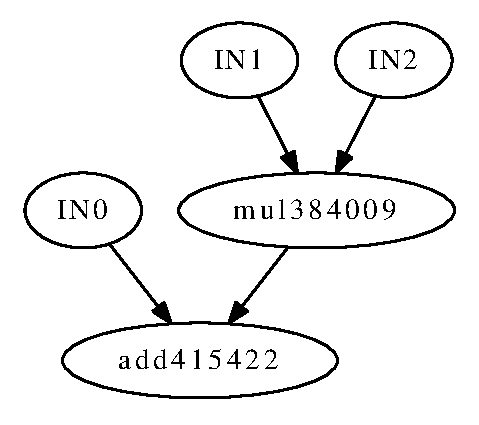
\includegraphics[width=2.5in]{source}
\caption{Graph representation of \texttt{add(IN0, mul(IN1,IN2))}}
\label{source_graph}
\end{figure}

\begin{figure*}
\centering
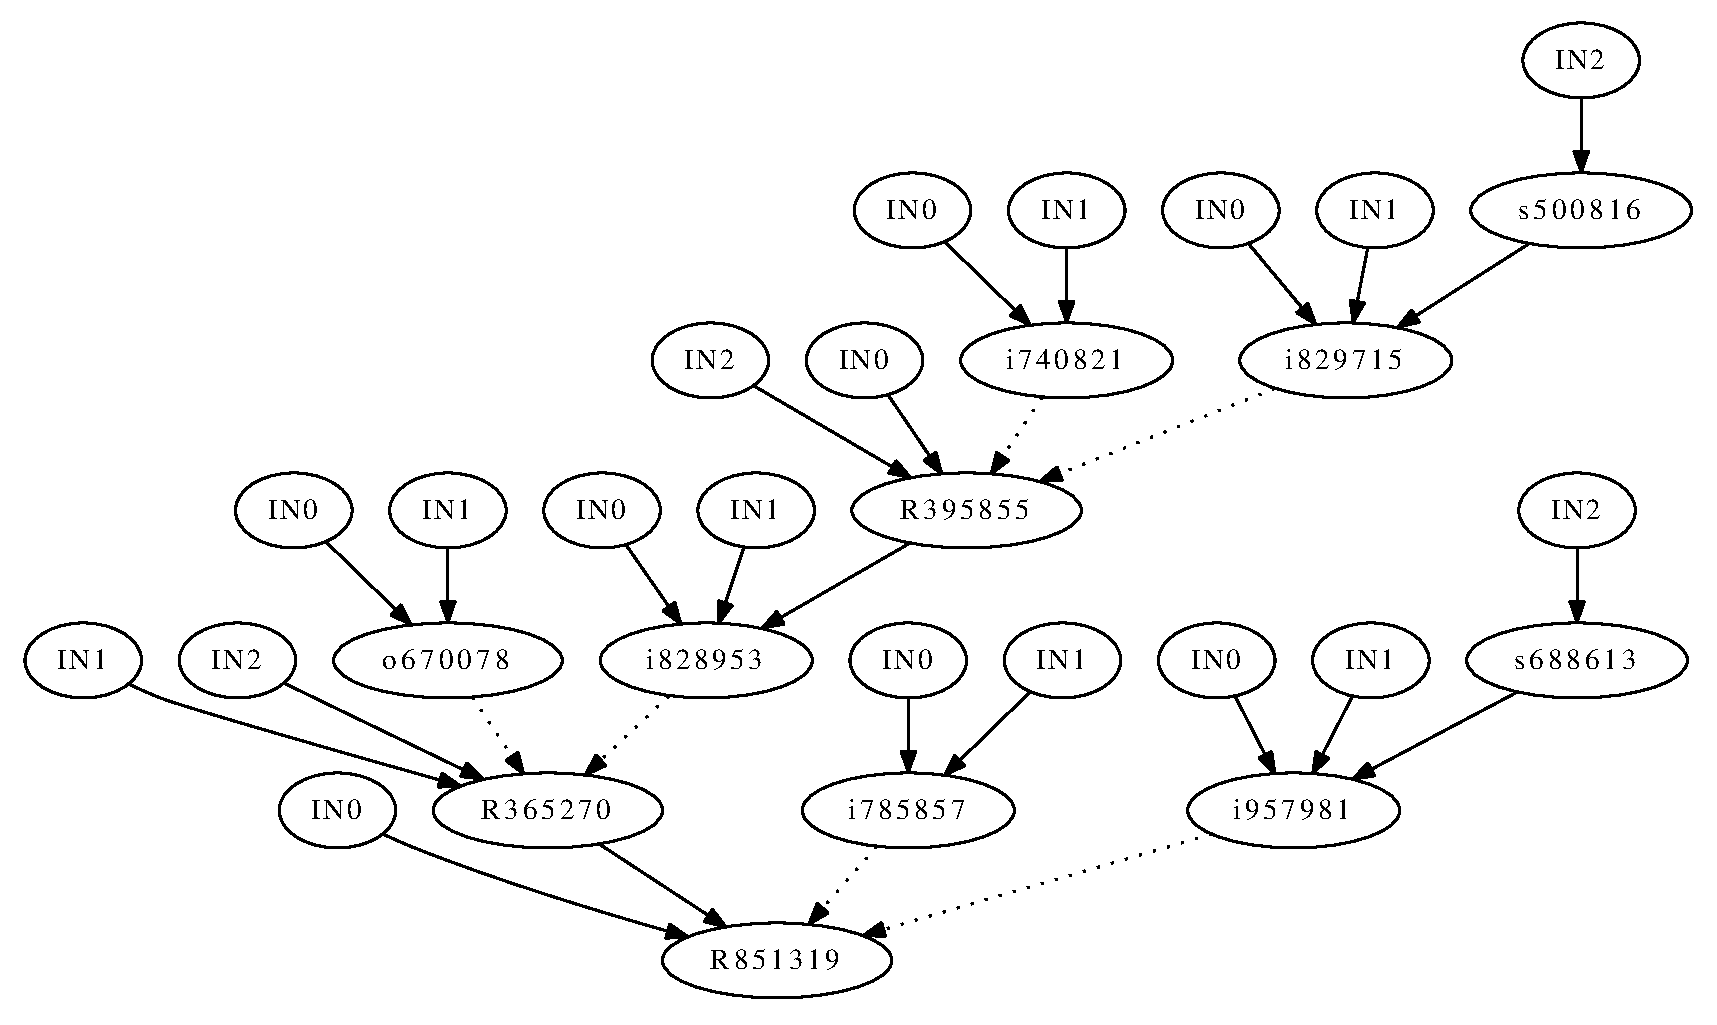
\includegraphics[width=6in]{primitive}
\caption{Graph representation of \texttt{add(IN0, mul(IN1,IN2)) after substitution.}}
\label{primitive_graph}
\end{figure*}

For convenience the system produces tree representation of expression  (fig. ~\ref{source_graph}). It has some non-terminal vertices computer not familiar with, but algorithm of the system can replace them substituting instead non-familiar non-terminal vertices compositions of familiar ones(fig. ~\ref{primitive_graph}). Such compositions represented in JSON format too. For example operation of addition in terms of Church algebra:\\
\texttt{
\{\\
\indent name:R,\\
\indent id:\%ID1\%,\\
\indent static:[\\
\indent \{\\
\indent \indent name:i,\\
\indent \indent id:\%ID2\%,\\
\indent \indent static:[0],\\
\indent \indent arguments:[\\
\indent \indent \indent \{no:0, value:IN0\},\\
\indent \indent \indent \{no:1, value:IN1\}\\
\indent \indent ]\\
\indent \},\\
\indent \{\\
\indent \indent name:i,\\
\indent \indent id:\%ID3\%,\\
\indent \indent static:[2],\\
\indent \indent arguments:[\\
\indent \indent \indent \{no:0, value:IN0\},\\
\indent \indent \indent \{no:1, value:IN1\},\\
\indent \indent \indent \{no:2, value:\{\\
\indent \indent \indent \indent name:s,\\
\indent \indent \indent \indent id:\%ID4\%,\\
\indent \indent \indent \indent static:[],\\
\indent \indent \indent \indent arguments:[\\
\indent \indent \indent \indent \indent \{no:0, value:IN2\}\\
\indent \indent \indent \indent ]\\
\indent \indent \indent \indent \}\\
\indent \indent \indent \}\\
\indent \indent ]\\
\indent \}\\
\indent ],\\
\indent arguments:[\\
\indent \indent \{no:0, value:\%IN0\%\},\\
\indent \indent \{no:1, value:\%IN1\%\}\\
\indent ] \\
\}\\
}
Dotted lines on the figure~\ref{primitive_graph} denote that child vertex is a static parameter. Vertices with names starting with ``o'' are zero generators. Vertices with names starting with ``s'' perform operation of increment. Vrtices with name starting with ``i'' perform operation of selection one of arguments to send it to output, using static parameter, hich denotes index of selected argument. Vertices with names starting with ``R'' represent primitive recursion composition. Terminal vertexes with names starting with ``IN'' represent arguments of the function in case when when a path from root to duch terminal vertex constists only of solid lines, in other case these are local inputs of compostion's static parameters.\\
The system produces HDL representation from such tree. To prove universality of the system, I have added generation of x86\_64 assembly as well. The system developed with Python programming language. It is agile enough to modify the system quickly.

% An example of a floating figure using the graphicx package.
% Note that \label must occur AFTER (or within) \caption.
% For figures, \caption should occur after the \includegraphics.
% Note that IEEEtran v1.7 and later has special internal code that
% is designed to preserve the operation of \label within \caption
% even when the captionsoff option is in effect. However, because
% of issues like this, it may be the safest practice to put all your
% \label just after \caption rather than within \caption{}.
%
% Reminder: the "draftcls" or "draftclsnofoot", not "draft", class
% option should be used if it is desired that the figures are to be
% displayed while in draft mode.
%
%\begin{figure}[!t]
%\centering
%\includegraphics[width=2.5in]{myfigure}
% where an .eps filename suffix will be assumed under latex, 
% and a .pdf suffix will be assumed for pdflatex; or what has been declared
% via \DeclareGraphicsExtensions.
%\caption{Simulation Results}
%\label{fig_sim}
%\end{figure}

% Note that IEEE typically puts floats only at the top, even when this
% results in a large percentage of a column being occupied by floats.


% An example of a double column floating figure using two subfigures.
% (The subfig.sty package must be loaded for this to work.)
% The subfigure \label commands are set within each subfloat command, the
% \label for the overall figure must come after \caption.
% \hfil must be used as a separator to get equal spacing.
% The subfigure.sty package works much the same way, except \subfigure is
% used instead of \subfloat.
%
%\begin{figure*}[!t]
%\centerline{\subfloat[Case I]\includegraphics[width=2.5in]{subfigcase1}%
%\label{fig_first_case}}
%\hfil
%\subfloat[Case II]{\includegraphics[width=2.5in]{subfigcase2}%
%\label{fig_second_case}}}
%\caption{Simulation results}
%\label{fig_sim}
%\end{figure*}
%
% Note that often IEEE papers with subfigures do not employ subfigure
% captions (using the optional argument to \subfloat), but instead will
% reference/describe all of them (a), (b), etc., within the main caption.


% An example of a floating table. Note that, for IEEE style tables, the 
% \caption command should come BEFORE the table. Table text will default to
% \footnotesize as IEEE normally uses this smaller font for tables.
% The \label must come after \caption as always.
%
%\begin{table}[!t]
%% increase table row spacing, adjust to taste
%\renewcommand{\arraystretch}{1.3}
% if using array.sty, it might be a good idea to tweak the value of
% \extrarowheight as needed to properly center the text within the cells
%\caption{An Example of a Table}
%\label{table_example}
%\centering
%% Some packages, such as MDW tools, offer better commands for making tables
%% than the plain LaTeX2e tabular which is used here.
%\begin{tabular}{|c||c|}
%\hline
%One & Two\\
%\hline
%Three & Four\\
%\hline
%\end{tabular}
%\end{table}


% Note that IEEE does not put floats in the very first column - or typically
% anywhere on the first page for that matter. Also, in-text middle ("here")
% positioning is not used. Most IEEE journals/conferences use top floats
% exclusively. Note that, LaTeX2e, unlike IEEE journals/conferences, places
% footnotes above bottom floats. This can be corrected via the \fnbelowfloat
% command of the stfloats package.



%%%%%%%%%%%%%%%%%%%%%%%%%%%%%%%%%%%%%%%%%%%%%%%%%%%%%%%%%
\section{Conclusion}
The described approach has a long history, but means to implement it and need in it emerged only nowadays. The state of microelectronic industry requires reconfigurable logic as one of the possible ways to avoid crysis which may come with the end of the Moore's low. A software proposed in the paper to compile sematic representation of problem's solution to syntax representation plays an important role in the approach, as one of the parts of it, which could be fully automated. The software is a proof of concept rather the one which ready for use in the industry, but it demonstrates ability to remove margin between software and hardware compiling the same semantic description of problem's solution into x86 assembly snd Verilog code. I believe that the approach will produce more reliable hardware and software, and will increase portability.


% conference papers do not normally have an appendix




% trigger a \newpage just before the given reference
% number - used to balance the columns on the last page
% adjust value as needed - may need to be readjusted if
% the document is modified later
%\IEEEtriggeratref{8}
% The "triggered" command can be changed if desired:
%\IEEEtriggercmd{\enlargethispage{-5in}}

% references section

% can use a bibliography generated by BibTeX as a .bbl file
% BibTeX documentation can be easily obtained at:
% http://www.ctan.org/tex-archive/biblio/bibtex/contrib/doc/
% The IEEEtran BibTeX style support page is at:
% http://www.michaelshell.org/tex/ieeetran/bibtex/
%\bibliographystyle{IEEEtran}
% argument is your BibTeX string definitions and bibliography database(s)
%\bibliography{IEEEabrv,../bib/paper}
%
% <OR> manually copy in the resultant .bbl file
% set second argument of \begin to the number of references
% (used to reserve space for the reference number labels box)

\bibliographystyle{IEEEtran}
\bibliography{pragmatic_dependent}{}


\end{document}


